\section{Resource-Constrained Data Loading}
\label{sec:data_loading}
Handling a dataset of planetary scale introduces a classic Big Data engineering challenge: the total volume of processed data often exceeds the available Random Access Memory (RAM).
Attempting to load the entire dataset of high-resolution float32 tensors into memory would result in immediate system exhaustion (Out-Of-Memory errors).
To address this, a \textbf{Resource-Constrained Data Loading} architecture was implemented within the \texttt{MapDataset} class, leveraging lazy loading, memory-aware chunking, and incremental caching.

\subsection{Chunk-Based Memory Management}
Naive implementations often attempt to allocate a single contiguous memory block for the entire dataset, leading to memory fragmentation and OOM errors on consumer hardware.
The \texttt{MapDataset} instead structures the data as a list of independent tensor chunks (\texttt{self.data\_real}, \texttt{self.data\_sim}).
During the dataset construction phase, a \texttt{consolidate\_and\_free\_memory} routine monitors the process's Resident Set Size (RSS).
When memory usage exceeds a safety threshold (e.g., 4GB), the accumulated patches are consolidated into a tensor chunk and appended to the main list.
Crucially, the temporary build buffer is then explicitly cleared and the system's garbage collector is manually invoked.
This aggressive memory reclamation ensures that unreferenced data is immediately freed rather than waiting for background automated processes, preventing sudden memory spikes and allowing the system to process datasets arbitrarily larger than the available physical RAM.

\begin{figure}[htbp]
    \centering
    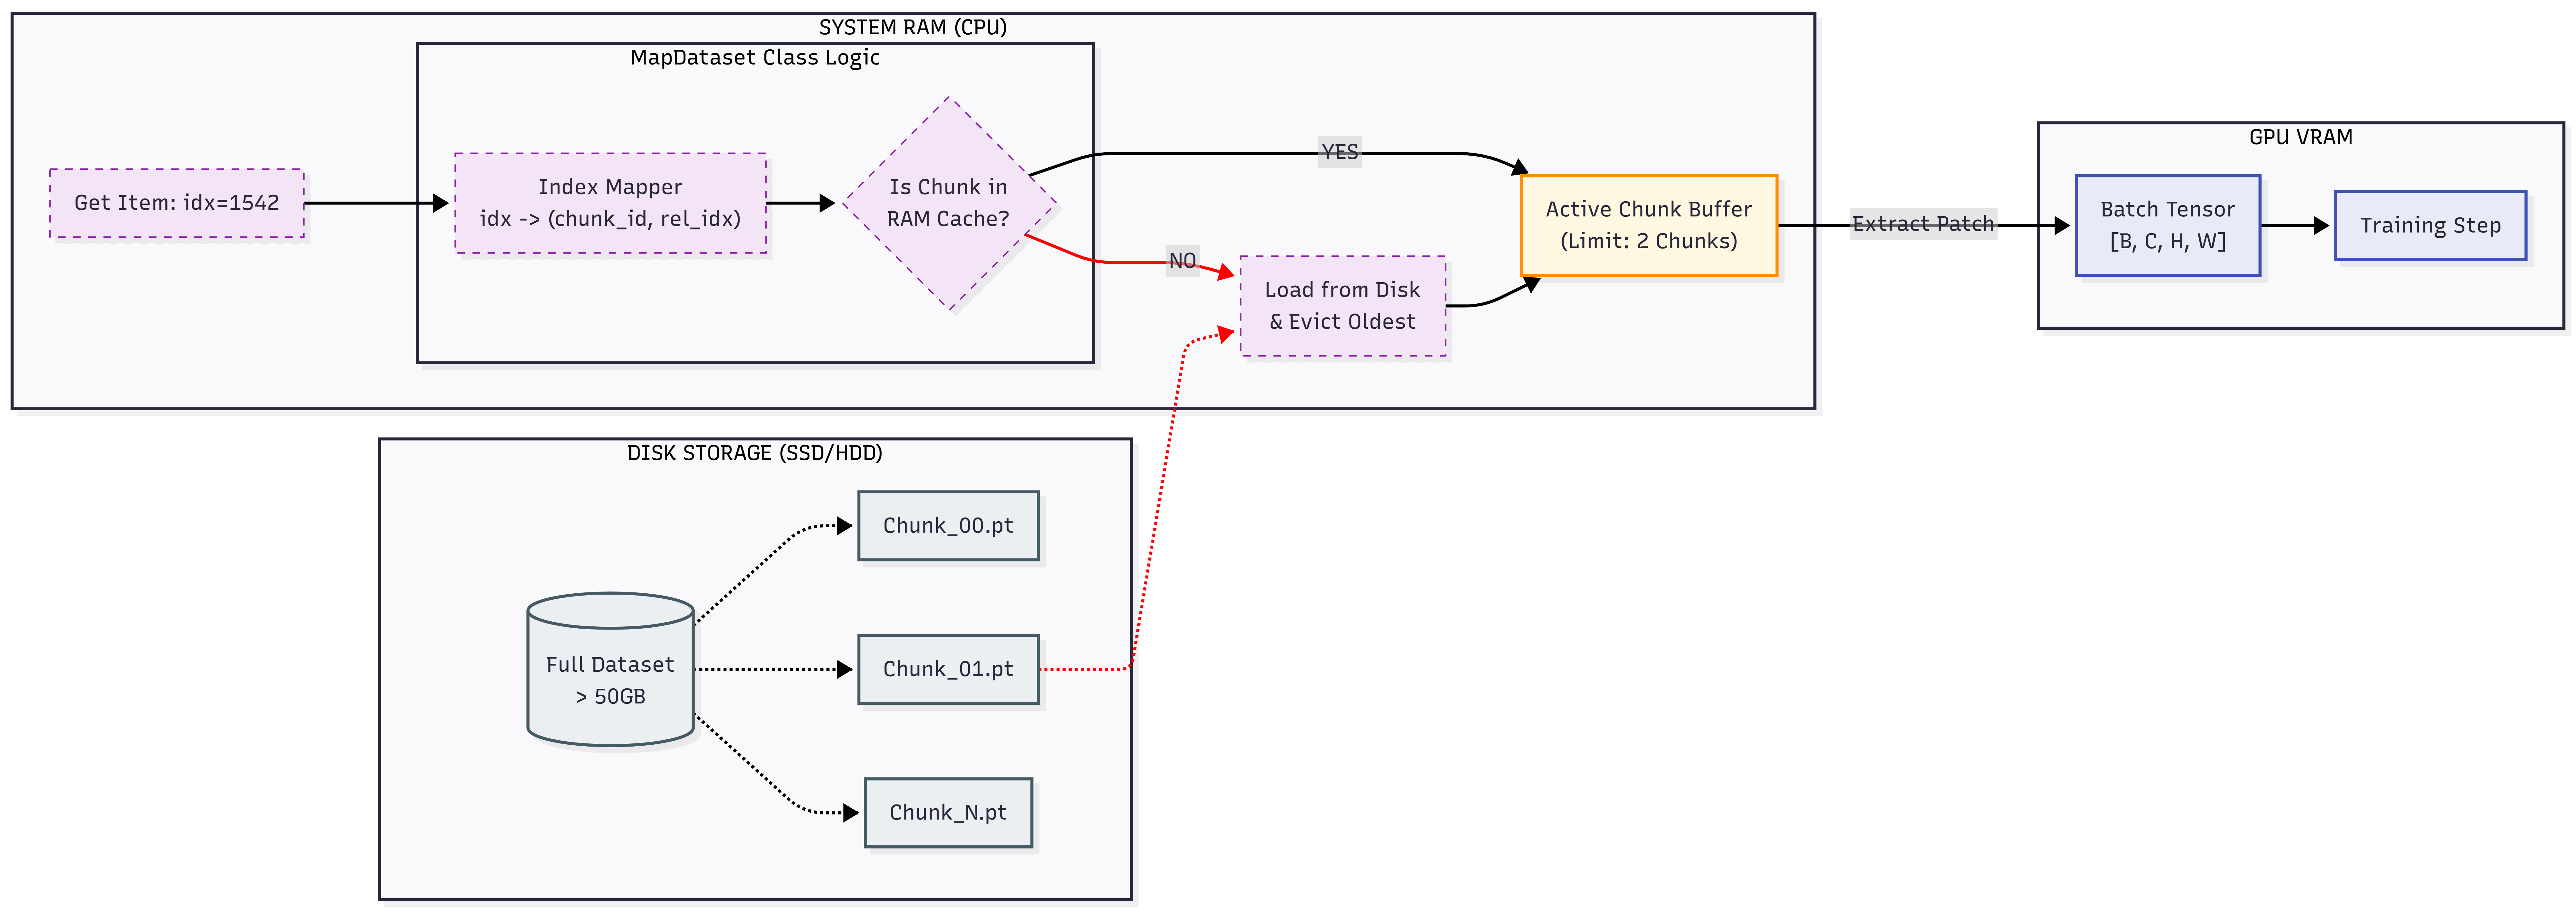
\includegraphics[width=\textwidth]{images/diagrams/memory-efficient-data-loading-strategy.png}
    \caption{Detail of the memory-efficient data loading strategy implemented in the MapDataset class. Large datasets are split into binary chunks on disk and dynamically loaded into a limited RAM buffer using a Least Recently Used (LRU) caching policy to enable training on consumer-grade hardware.}
    \label{fig:data_loading_strategy}
\end{figure}

\subsection{Two-Pass Incremental Build and Caching}
To eliminate the overhead of repeated pre-processing, the system implements a \textbf{Caching Mechanism}.
The \texttt{two\_pass\_incremental\_build} function orchestrates the dataset creation using a two-pass algorithm designed to minimize peak memory usage:

\begin{enumerate}
    \item \textbf{Pass 1 (Statistics):} The pipeline iterates through the entire raw dataset on disk to compute global normalization statistics (global Min/Max) without storing the images in memory. This ensures that the subsequent normalization is consistent across the entire dataset.
    \item \textbf{Pass 2 (Extraction):} The pipeline re-iterates to apply normalization and extract patches using the computed statistics. This phase utilizes a "streaming" approach, where patches are extracted, accumulated in chunks, and serialized to disk as independent \texttt{.pt} (PyTorch) binary archives.
\end{enumerate}

\subsection{Disk Caching and LRU Dynamic Loading Strategy}
For subsequent training runs, the system calculates a hash (MD5) of the current configuration (patch size, normalization type, etc.).
If the corresponding cache files matching this hash exist, the dataset is loaded directly from disk (\texttt{load\_from\_cache}), bypassing the raw data processing entirely.
This reduction in startup time—from hours to seconds—is critical for rapid experimental iteration.

Once the data is serialized into independent binary chunks on disk, their dynamic loading during the training phase is governed by a \textbf{Least Recently Used (LRU) caching policy}.
Instead of keeping all chunks in memory simultaneously, the \texttt{MapDataset} maintains a strictly bounded RAM buffer.
When a specific data patch is requested by the Dataloader, the system checks if its parent chunk is currently in the RAM cache.
If a cache miss occurs, the chunk is sequentially loaded from disk.
Should the RAM buffer be at maximum capacity, the LRU algorithm automatically deallocates the chunk that has not been accessed for the longest time, making room for the new one.
This strategy guarantees fast batch generation while keeping the memory footprint strictly within consumer-grade hardware limits.

